\documentclass[11pt]{article}

\usepackage{pdflscape}
\usepackage{graphicx}
\usepackage[hidelinks]{hyperref}

\begin{document}

\begin{titlepage}
	\begin{center}
		
		\begin{figure}[t]
			\centering
			
\includegraphics[width=350px]{../Images/UP_Logo.png}
		\end{figure}
		
		% Title
		\textsc{\large } \\ 
		\vspace{2cm}
		\textbf{\Huge IMY 310 Project  \\
			Project Plan \\
			(Phase 1)} \\ 

		\textsc{\large } \\ 
		\vspace{0.75cm}

		\textbf{\Large AgriSales Magazine} \\ 
		
		\begin{flushright} \large
			Azhar Mohungoo \emph{12239799} \newline
			Daniel Malangu \emph{} \newline
			Kudzai  	\emph{} \newline
			\newline
			Group Name  \emph{} \newline
			\end{flushright}
		%\end{minipage}
		
	\end{center}
\end{titlepage}


\tableofcontents

\listoffigures

\newpage

\section{Paper Prototype Designs}
	
	\subsection{Original Designs}
	
	\subsubsection{Home Page}
		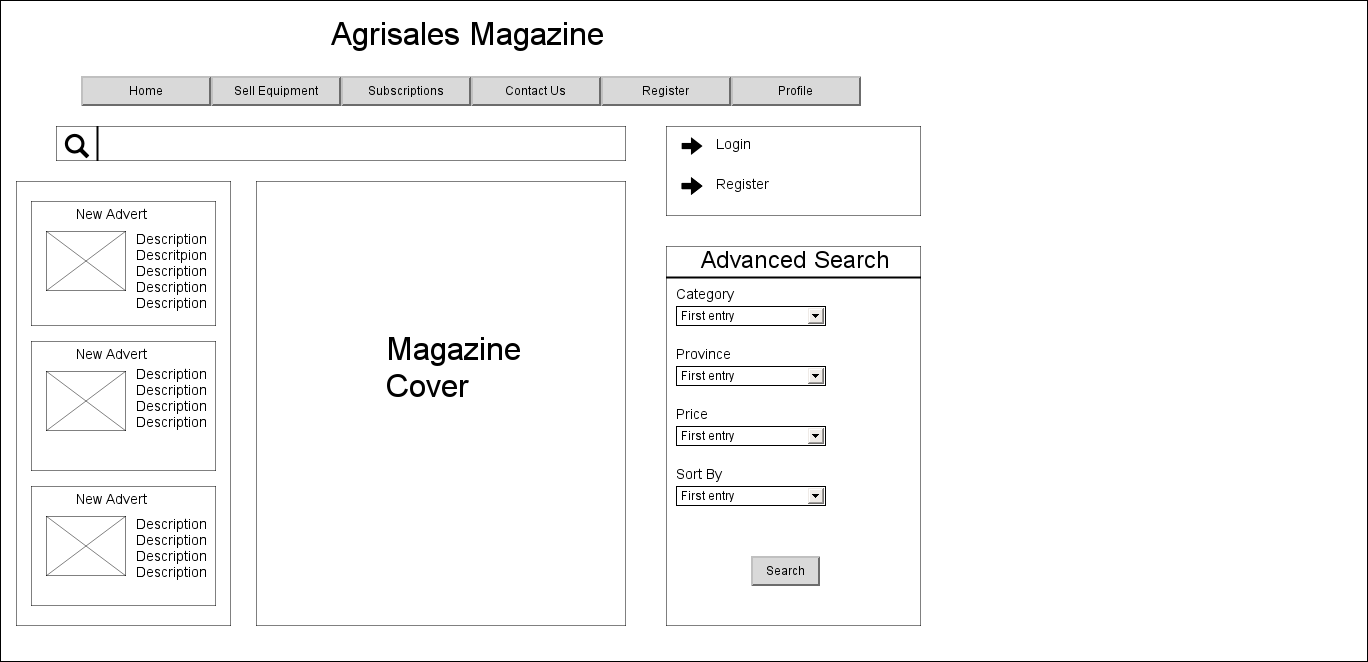
\includegraphics[width=0.75\linewidth]{../Images/Agrisales-HomePage}
		
	\subsubsection{Login Page}
		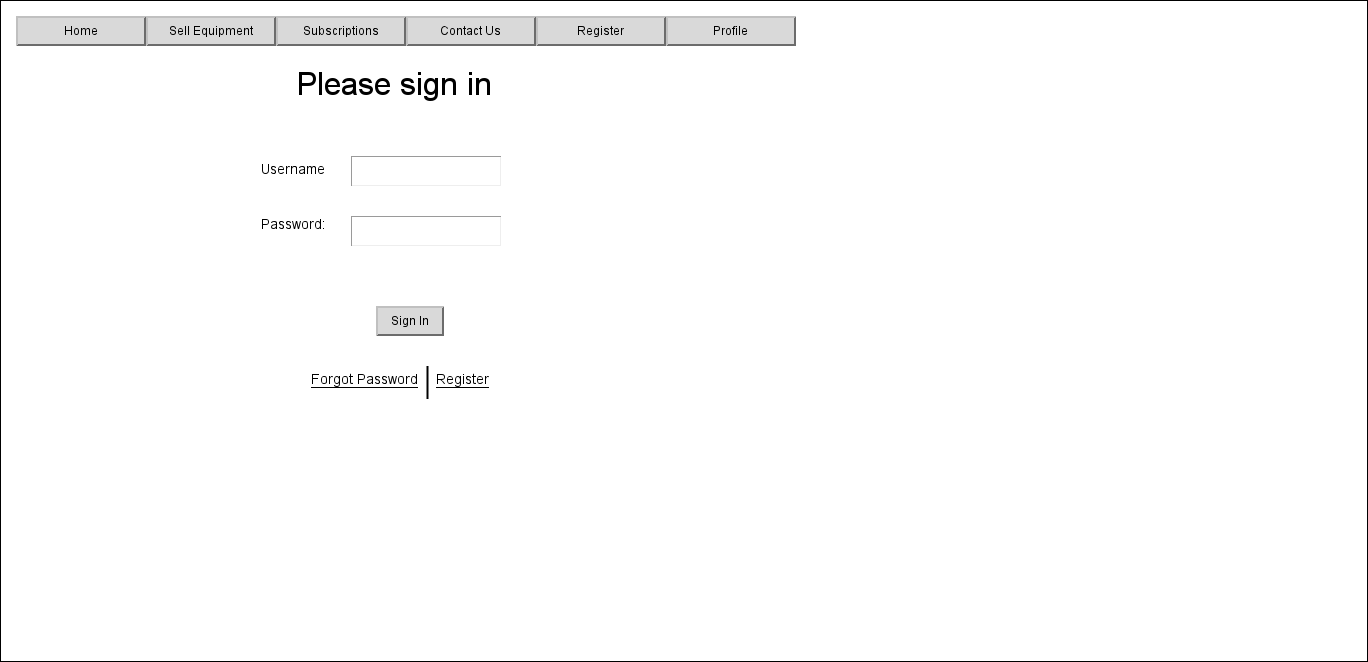
\includegraphics[width=0.75\linewidth]{../Images/Agrisales-LoginPage}
		
	\subsubsection{Registration Page}
		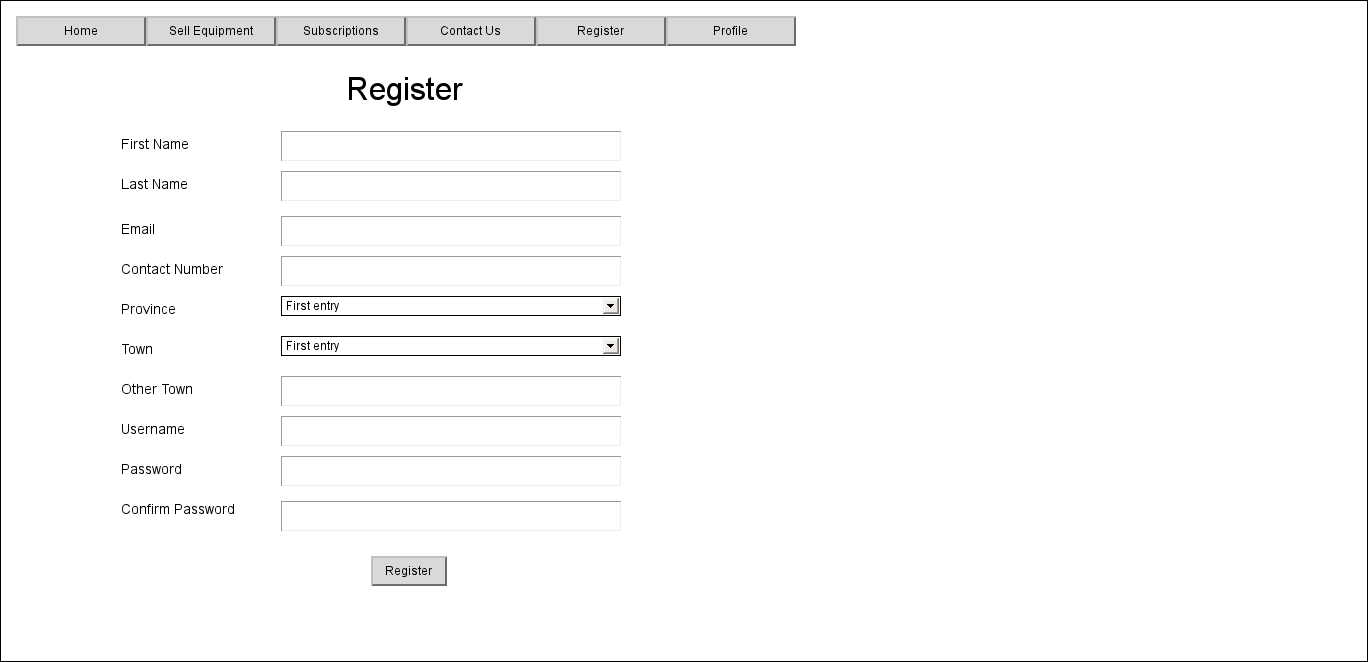
\includegraphics[width=0.75\linewidth]{../Images/Agrisales-RegistrationPage}
		
	\subsubsection{Advertisements Page}
		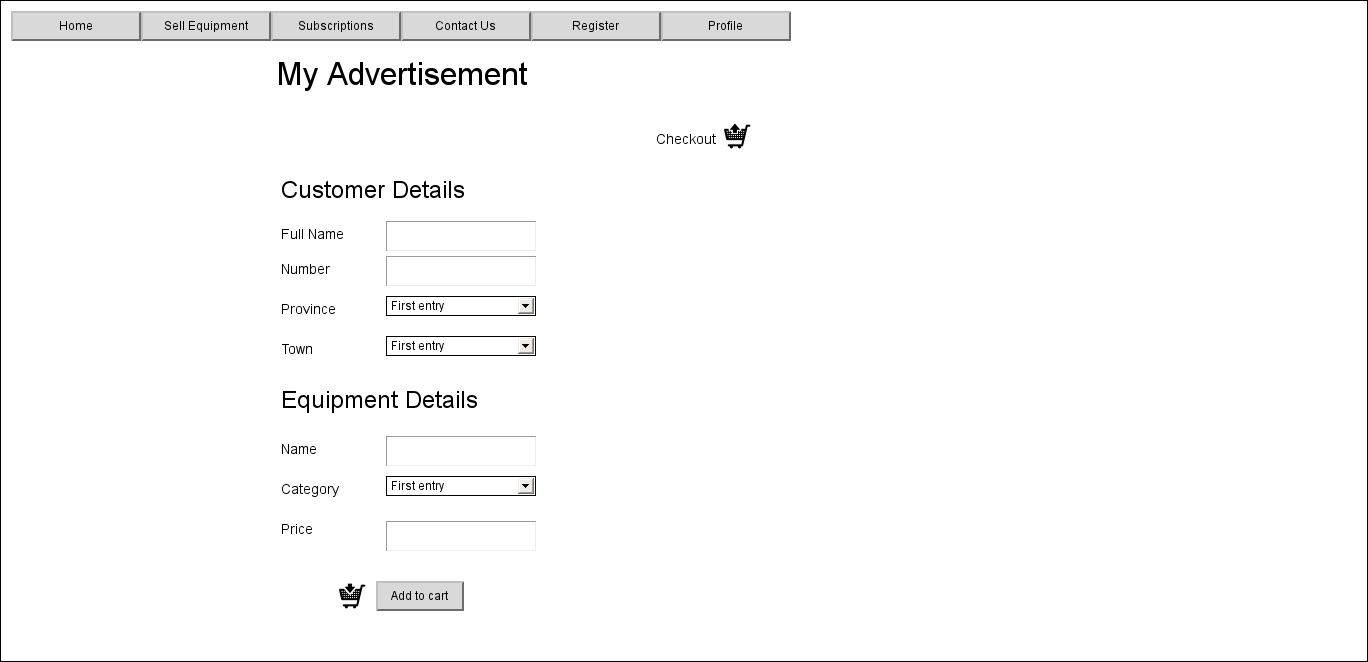
\includegraphics[width=0.75\linewidth]{../Images/Agrisales-AdvertisementsPage}
		
	\subsubsection{Subscriptions Page}
		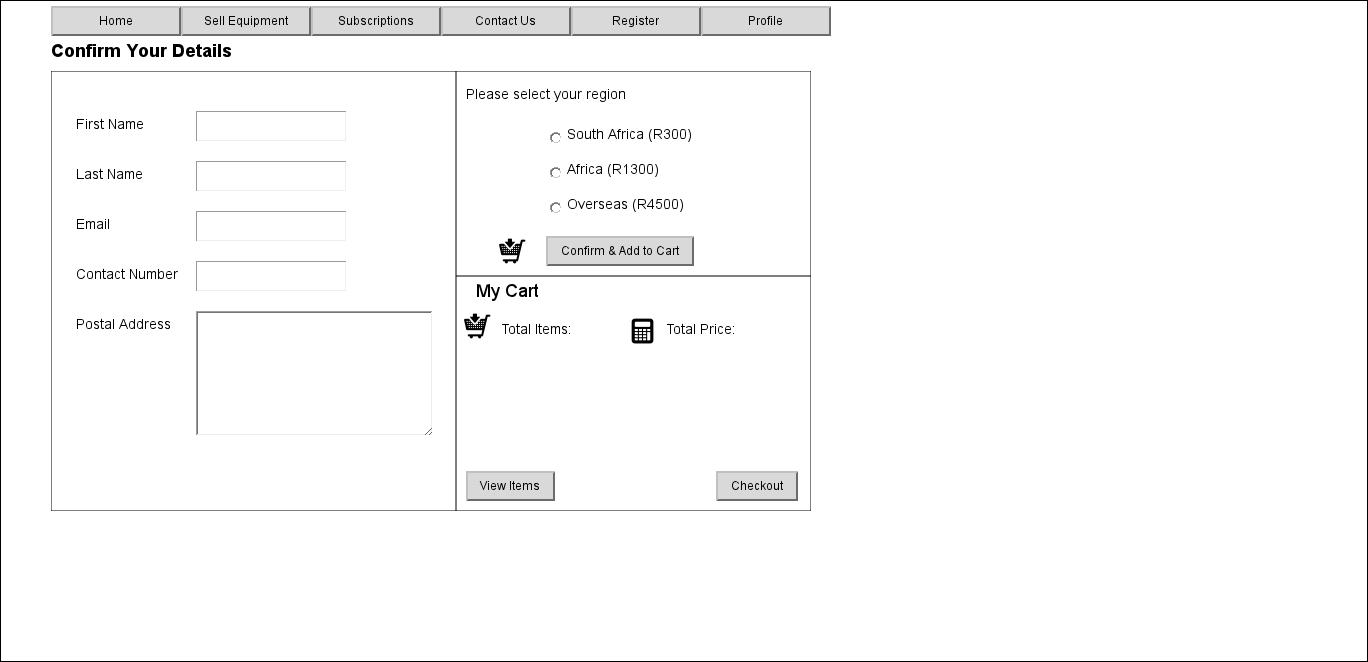
\includegraphics[width=0.75\linewidth]{../Images/AgriSales-SubscriptionsPage}
		
	\subsubsection{View Ad Page}
		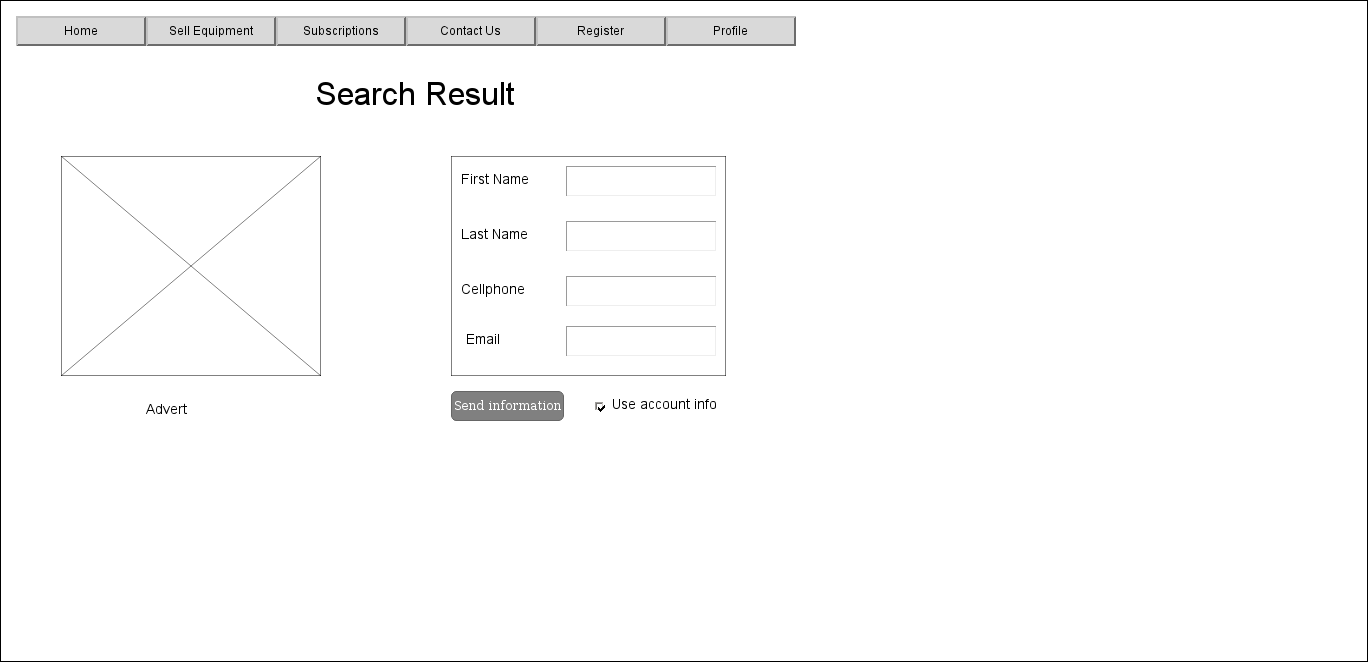
\includegraphics[width=0.75\linewidth]{../Images/AgriSales-ViewAdPage}
		
	\subsubsection{Contact Us Page}
		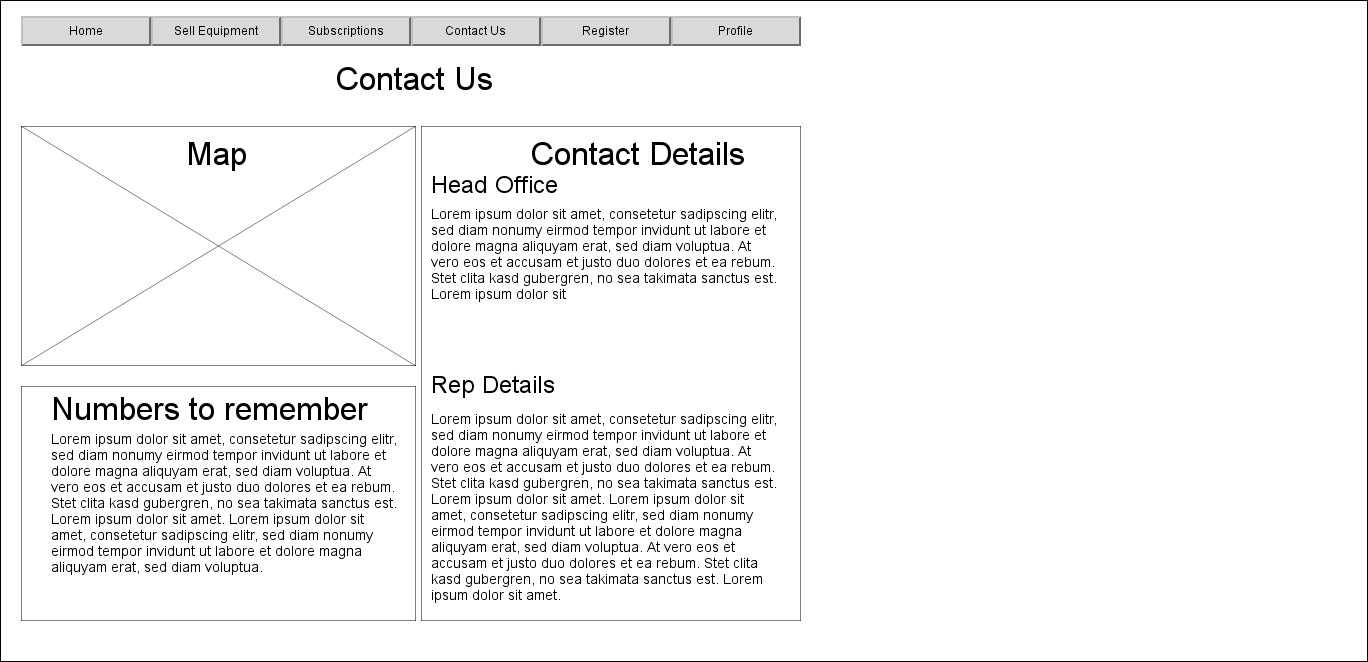
\includegraphics[width=0.75\linewidth]{../Images/Agrisales-ContactUsPage}
		
	\subsubsection{Alternative Home Page}
		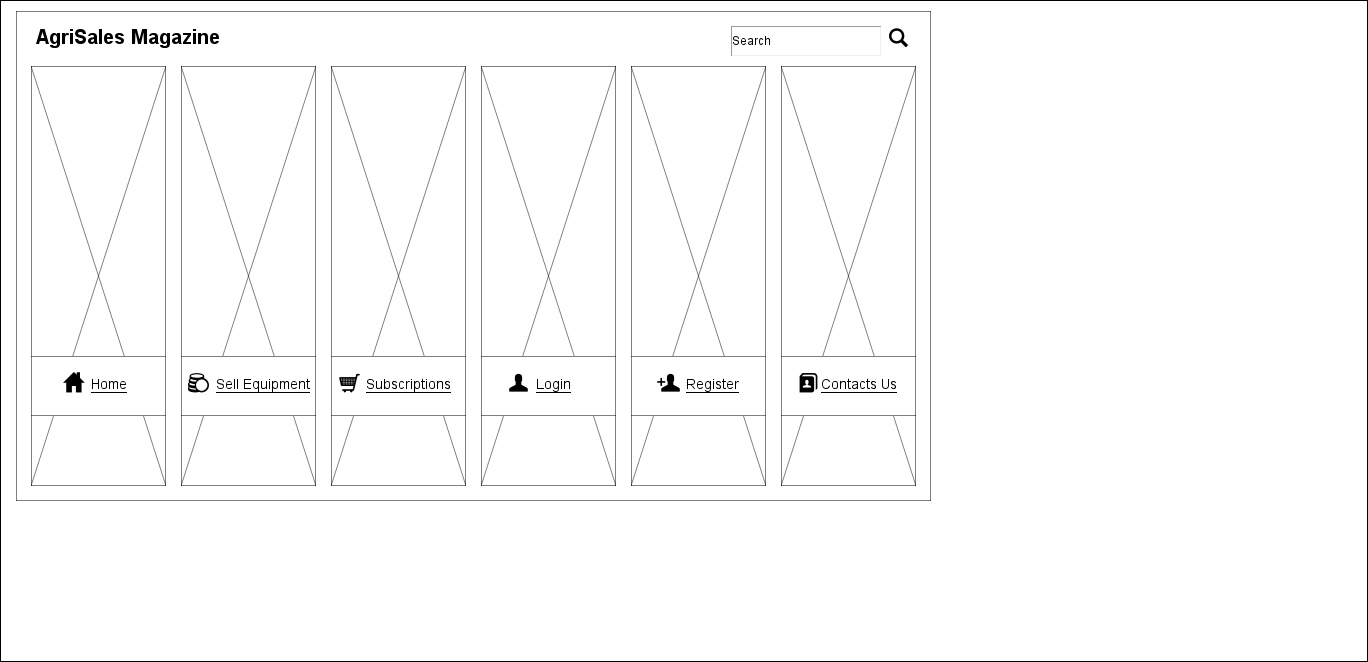
\includegraphics[width=0.75\linewidth]{../Images/AgriSales-AlternativeHomePage}
		
	\subsubsection{Alternative Advertisement Page}
		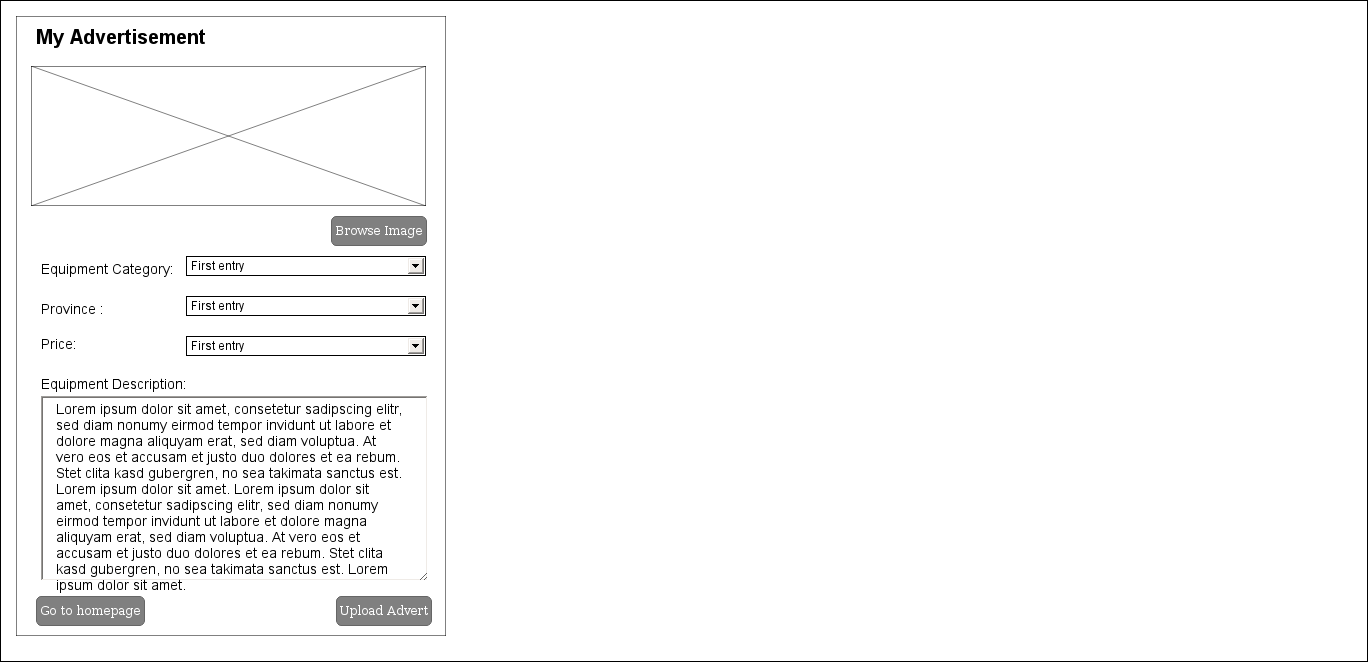
\includegraphics[width=0.75\linewidth]{../Images/AgriSales-AlternativeAdvertisementPage}
		
	\subsubsection{Alternative Subscriptions Page}
		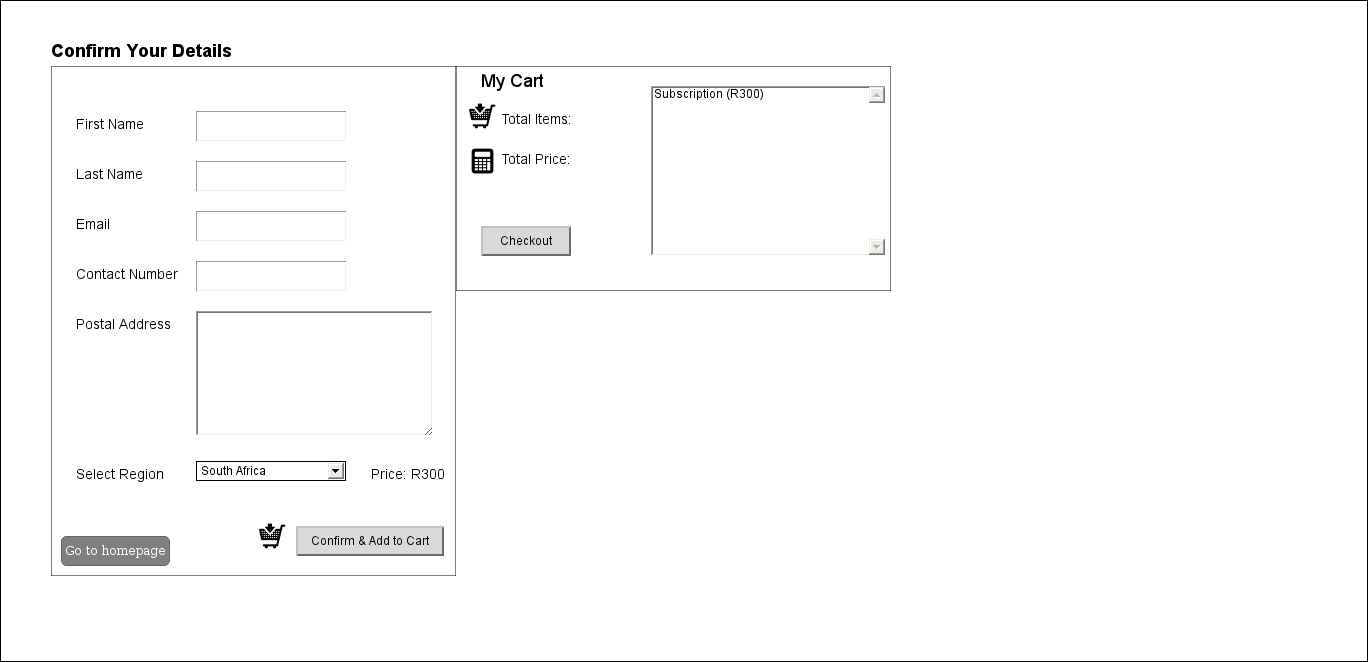
\includegraphics[width=0.75\linewidth]{../Images/AgriSales-AlternativeSubscriptionsPage}
		
	\subsubsection{Alternative Contact Us Page}
		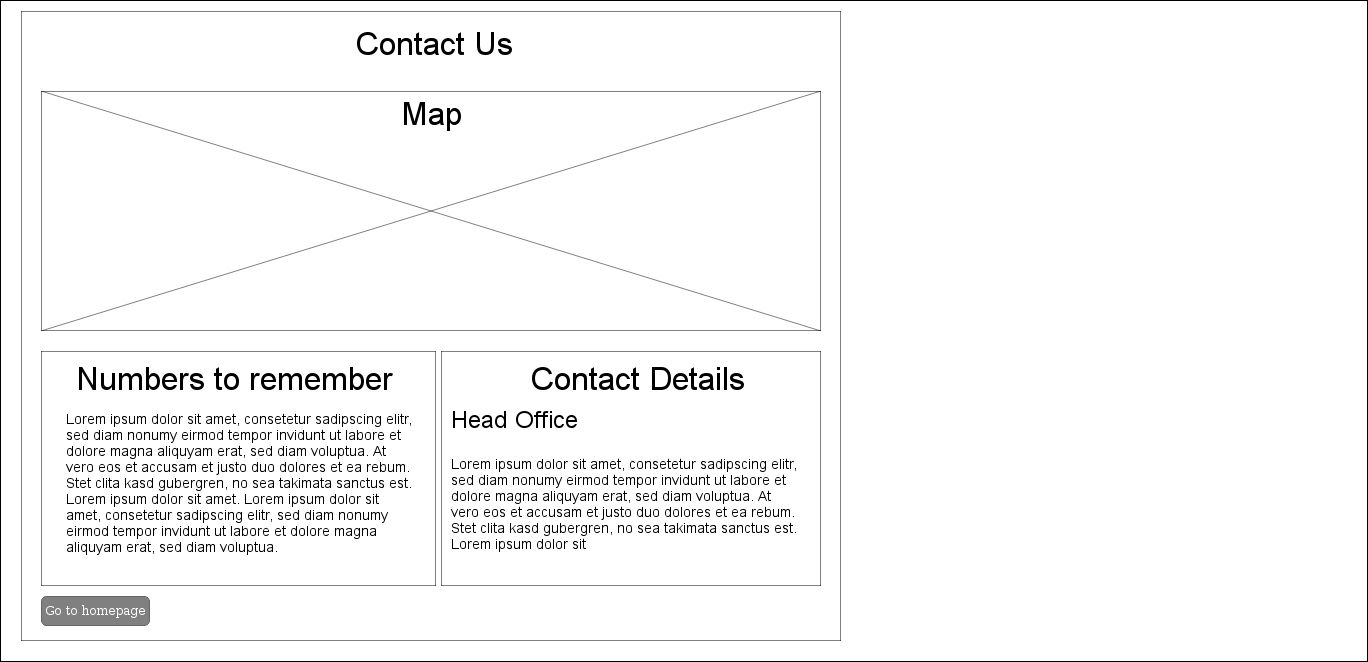
\includegraphics[width=0.75\linewidth]{../Images/AgriSale-AlternativeContactUsPage}

\newpage

\section{Motivations for Alternative Designs}

\section{Testing the Designs}
	When testing, we presented our paper based designs to the stakeholders in a sequential order starting from the home page. We proceeded to each of the options within the menu of the home page, while providing them with explanations on how the product functions moving from one web page to the other. The stakeholders then provided us with comments about the sketches, which in turn helps us determine what they expect and what changes they would like to make for the product.

\section{Feedback Received}

\section{Using the Feedback}
	
\end{document}
